%%
%% getstart.tex -- Flight Gear documentation: Installation and Getting Started
%% Chapter file
%%
%% Written by Bernhard Buckel, starting September 1998.
%%
%% Copyright (C) 1999  Bernhard Buckel (buckel@wmad95.mathematik.uni-wuerzburg.de)
%%
%% This program is free software; you can redistribute it and/or
%% modify it under the terms of the GNU General Public License as
%% published by the Free Software Foundation; either version 2 of the
%% License, or (at your option) any later version.
%%
%% This program is distributed in the hope that it will be useful, but
%% WITHOUT ANY WARRANTY; without even the implied warranty of
%% MERCHANTABILITY or FITNESS FOR A PARTICULAR PURPOSE.  See the GNU
%% General Public License for more details.
%%
%% You should have received a copy of the GNU General Public License
%% along with this program; if not, write to the Free Software
%% Foundation, Inc., 675 Mass Ave, Cambridge, MA 02139, USA.
%%
%% $Id: getstart.tex,v 0.12 1999/03/07 michael


%%%%%%%%%%%%%%%%%%%%%%%%%%%%%%%%%%%%%%%%%%%%%%%%%%%%%%%%%%%%%%%%%%%%%%%%%%%%%%%%%%%%%%%%%%%%%%%%%
\chapter{Takeoff: How to start the program\label{takeoff}}
%%%%%%%%%%%%%%%%%%%%%%%%%%%%%%%%%%%%%%%%%%%%%%%%%%%%%%%%%%%%%%%%%%%%%%%%%%%%%%%%%%%%%%%%%%%%%%%%%
\markboth{\thechapter.\hspace*{1mm}
TAKEOFF}{\thesection\hspace*{1mm} Command line parameters}

\section{Starting under Linux}
Under Linux, \FlightGear is invoked by

  \texttt{fgfs -$\!$-option1 -$\!$-option2\dots},

\noindent
 where the options are described in section \ref{options} below.

\section{Starting under \Index{Windows 98/NT}}

In Windows explorer, change to \texttt{$\backslash$FlightGear$\backslash$}. Call
\texttt{runfgfs.bat} by double-clicking if you want to invoke the hardware accelerated
version of \FlightGear \texttt{fgfs.exe}, or \texttt{runfgfs-sgi.bat} if you installed
SGI's software \Index{OpenGL} support.

Alternatively, if for one or the other reason the batch does not work, you can open an
MS-DOS shell, change to the directory where your binary resides (typically something like
\texttt{d:$\backslash$FlightGear$\backslash$bin} where you might have to substitute
\texttt{d:} in favor of your \FlightGear directory), set the environment variable with

\texttt{SET FG\_ROOT=d:$\backslash$FlightGear$\backslash$bin}

\noindent
 and invoke \FlightGear (within the same shell -- Windows environment
 settings are only valid locally within the same shell) via

\texttt{fgfs -$\!$-option1 -$\!$-option2\dots}.

For getting maximum performance it is highly recommended to
minimize (iconize) the non-graphics window while running
{\FlightGear}$\!$.
 \medskip

 \centerline{
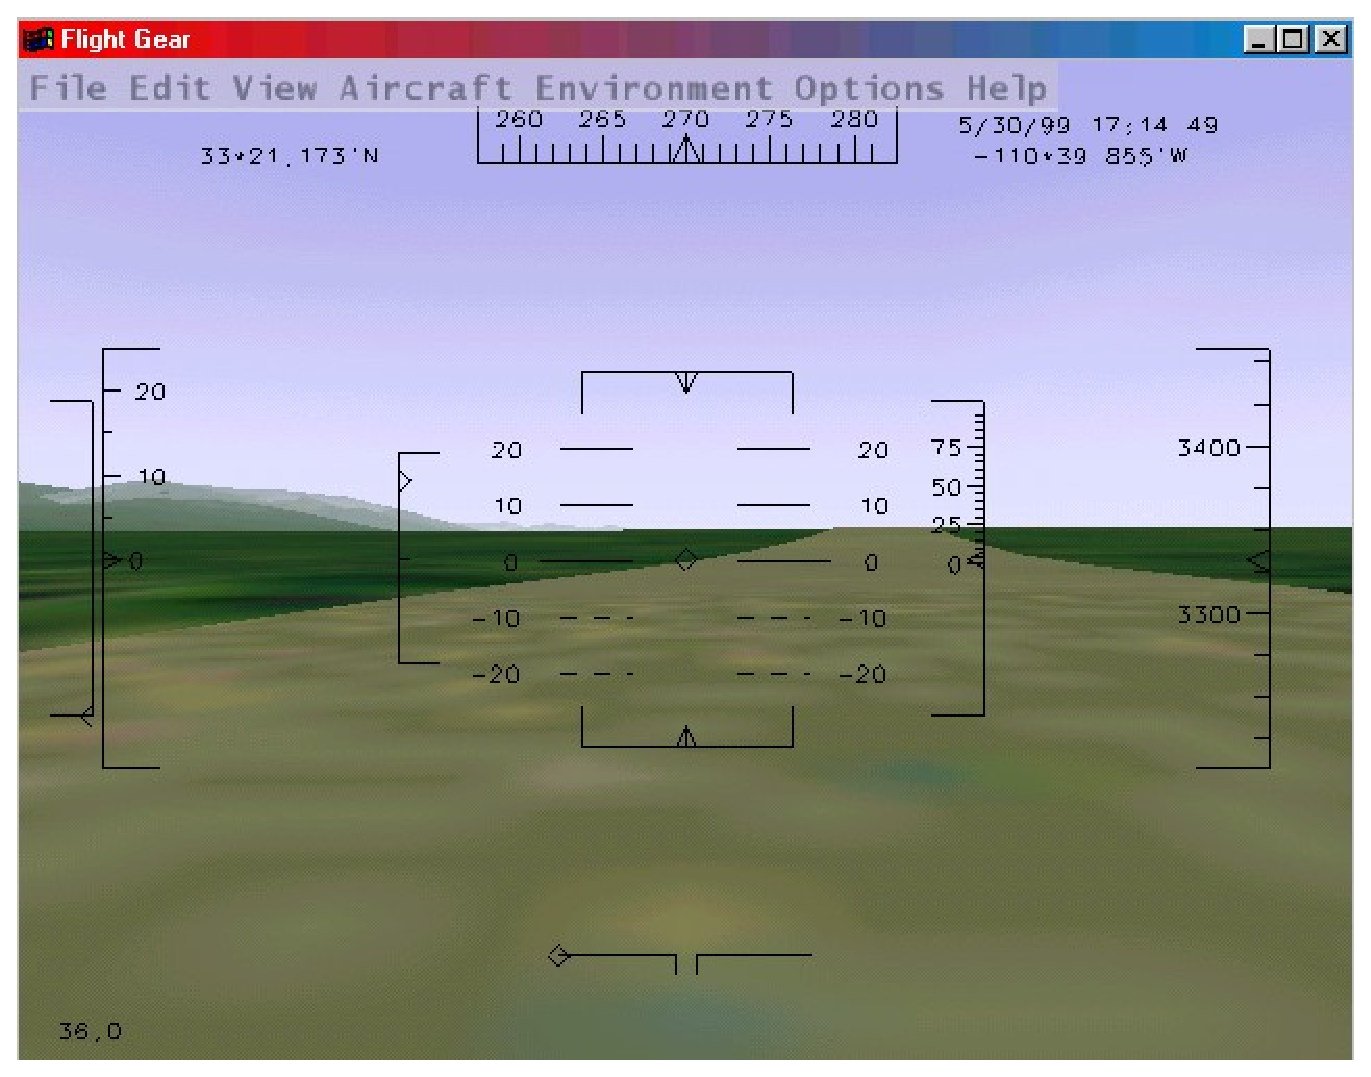
\includegraphics[clip,width=12.5cm]{arizona.eps}
}

 \noindent
Fig.\,2: \textit{Ready for takeoff. We are at the default startup
position in Arizona.}
\medskip

\section{Command line parameters\label{options}}
\index{command line options}

Following is a list and short description of the command line options available. In case
of Windows 98/NT it is recommended to include these in \texttt{runfgfs.bat}.

\subsection{General Options}

\begin{itemize}

\item{\texttt{-$\!$-help}}: gives a small help text, kind of a short version of this section.

\item{\texttt{-$\!$-fg-root={\it path}}}: tells \FlightGear where to look for its data
  files if you didn't compile it with the default settings.

\item{\texttt{-$\!$-disable-game-mode}}: Disables \Index{fullscreen display}.


\item{\texttt{-$\!$-enable-game-mode}}: Enables fullscreen rendering.


\item{\texttt{-$\!$-disable-splash-screen}}: Turns off the rotating \Index{3DFX
logo} when the accelerator board gets initialized.

\item{\texttt{-$\!$-enable-splash-screen}}: If you like advertising, set this!

\item{\texttt{-$\!$-disable-intro-music}}: No MP3-sample is being played when
  \FlightGear starts up.

\item{\texttt{-$\!$-enable-intro-music}}: If your machine is powerful enough, enjoy
  this setting.

\item{\texttt{-$\!$-disable-mouse-pointer}}: In the future, \FlightGear will
  feature a mouse interface so that options can be set at runtime.  As
  this feature is not implemented yet it seems wise to disable the
  mouse interface.

\item{\texttt{-$\!$-enable-mouse-pointer}}: Enables another mouse pointer in the
  \FlightGear window. This is useful when running \FlightGear in full
  screen mode and will allow access to the - yet to be implemented -
  mouse interface of \FlightGear\hspace{-2mm}.

\item{\texttt{-$\!$-disable-pause}}: This will put you into \FlightGear with the
  engine running, ready for Take-Off.

\item{\texttt{-$\!$-enable-pause}}: Starts \FlightGear in pause mode.

\end{itemize}

\subsection{Features}

\begin{itemize}

\item{\texttt{-$\!$-disable-hud}}: Switches off the \Index{HUD} (\textbf{H}ead \textbf{U}p
  \textbf{D}isplay).

\item{\texttt{-$\!$-enable-hud}}: Turns the  \Index{HUD} on. This is the default.

\item{\texttt{-$\!$-disable-panel}}: Turns off the \Index{instrument panel}. This is the
  default, as the instrument panel is still in its early beginnings -- but in our opinion
  you should give it a try.

\item{\texttt{-$\!$-enable-panel}}: This will give you the look of a real \Index{cockpit}.

\item{\texttt{-$\!$-disable-sound}}: Pretty self explaining, isn't it?

\item{\texttt{-$\!$-enable-sound}}:

\end{itemize}

\subsection{Initial Position and Orientation\index{orientation}}

\begin{itemize}

\item{\texttt{-$\!$-airport-id=ABCD}}: If you want to start directly at an airport,
  enter its international code, i.e. KJFK for JFK airport in New York.
  A long/short list of the IDs of the airports being implemented can
  be found in \texttt{/Flight Gear/Airports}. You only have to unpack
  one of the files with gnuzip. Keep in mind, you need the
  terrain data for the relevant region!\index{airport code}

\item{\texttt{-$\!$-lon=degrees}}: This is the starting longitude in degrees (west = -)

\item{\texttt{-$\!$-lat=degrees}}: This is the starting latitude in degrees (south = -)

\item{\texttt{-$\!$-altitude=meters}}: You may start in free flight at the given
  altitude. Watch for the next options to insert the plane with a
  given heading etc.

\item{\texttt{-$\!$-heading=degrees}}: Sets the \Index{initial heading}.

\item{\texttt{-$\!$-roll=degrees}}: Initial roll angle.\index{initial roll angle}

\item{\texttt{-$\!$-pitch=degrees}}: Initial pitch angle.\index{initial pitch angle}

\end{itemize}

\subsection{Rendering Options\index{rendering options}}

\begin{itemize}

\item{\texttt{-$\!$-fog-disable}}: To cut down the rendering efforts, distant
  regions are vanishing in \Index{fog} by default. If you disable fogging,
  you'll see farther but your frame rates will drop.

\item{\texttt{-$\!$-fog-fastest}}: The scenery will not look very nice but
  frame rates will increase.

\item{\texttt{-$\!$-fog-nicest}}: This option will give you a fairly realistic
  view of flying on a hazy day.

\item{\texttt{-$\!$-fov=xx.x}}: Sets the \Index{field of view} in degrees.
The value is displayed on the HUD. Default is 55.0.

\item{\texttt{-$\!$-disable-fullscreen}}: Self explaining, isn't it?

\item{\texttt{-$\!$-enable-fullscreen}}:

\item{\texttt{-$\!$-shading-flat}}: This is the fastest mode but the terrain will look ugly! This option might help if your video accelerator is really slow.

\item{\texttt{-$\!$-shading-smooth}}: This is the recommended (and default) setting - things will look really nice.

\item{\texttt{-$\!$-disable-skyblend}}: No fogging or \Index{haze}, sky will be displayed
  using just one color. Fast but ugly!

\item{\texttt{-$\!$-enable-skyblend}}: Fogging/haze is enabled, sky and \Index{terrain} look realistic. This is the default and recommended setting.

\item{\texttt{-$\!$-disable-textures}}: Terrain details will be disabled. Looks ugly, but might help if your video board is slow.

\item{\texttt{-$\!$-enable-textures}}: Default and recommended.

\item{\texttt{-$\!$-enable-wireframe}}: If you want to know how the world of \FlightGear internally looks like, try this!

\end{itemize}

%% Revision 0.02  1998/09/29  bernhard
%% revision 0.10  1998/10/01  michael
%% final proofreading for release
%% revision 0.11  1998/11/01  michael
%% Added pic from Arizona takeoff
